\section{The Road to Improving Angular Momentum Conservation in Arepo}
\label{sec:c3_fixingarepo}

The first simulation we performed in \arepo\ showed dramatic differences from our \gasoline\ ones.  In it, the $0.625\,\Msun$ donor WD is destroyed by tidal forces within $\sim3$ orbital periods ($\sim150\,\mrm{s}$), versus the \gasoline\ simulation's $\sim4$ ($\sim200\,\mrm{s}$).  Following coalescence, the \arepo\ simulation featured a dense, cresent-shaped region formed from accretor material, retaining its pre-merger temperature of $\sim10^7\,\mrm{K}$, while the \gasoline\ merger remnant was relatively hot throughout its interior, with an average temperature of $\sim2\times10^8\,\mrm{K}$.  Most prominently, the \gasoline\ remnant evolved into an axisymmetric configuration $\sim250$ s after coalescence while the \arepo\ remnant maintained the integrity of its non-axisymmetric crescent while launching one, and then multiple trailing spiral waves into the surrounding medium.  Over $\sim10^3\,\mrm{s}$, the angular velocity of the entire remnant dropped to zero.  Spiral waves -- hitherto unmentioned in WD merger literature (though frequently discussed in the context of accretion disks) -- are a mechanism for transporting angular momentum (eg. \citealt{papal95, balb03}) and was initially presumed to be the cause of this remnant spin-down.  Global angular momentum, however, was not conserved, and in this section we summarize our attempts at isolating the cause of this angular momentum leak, and which features discussed above turned out to be spurious once the leak was plugged.

\begin{figure}
\centering
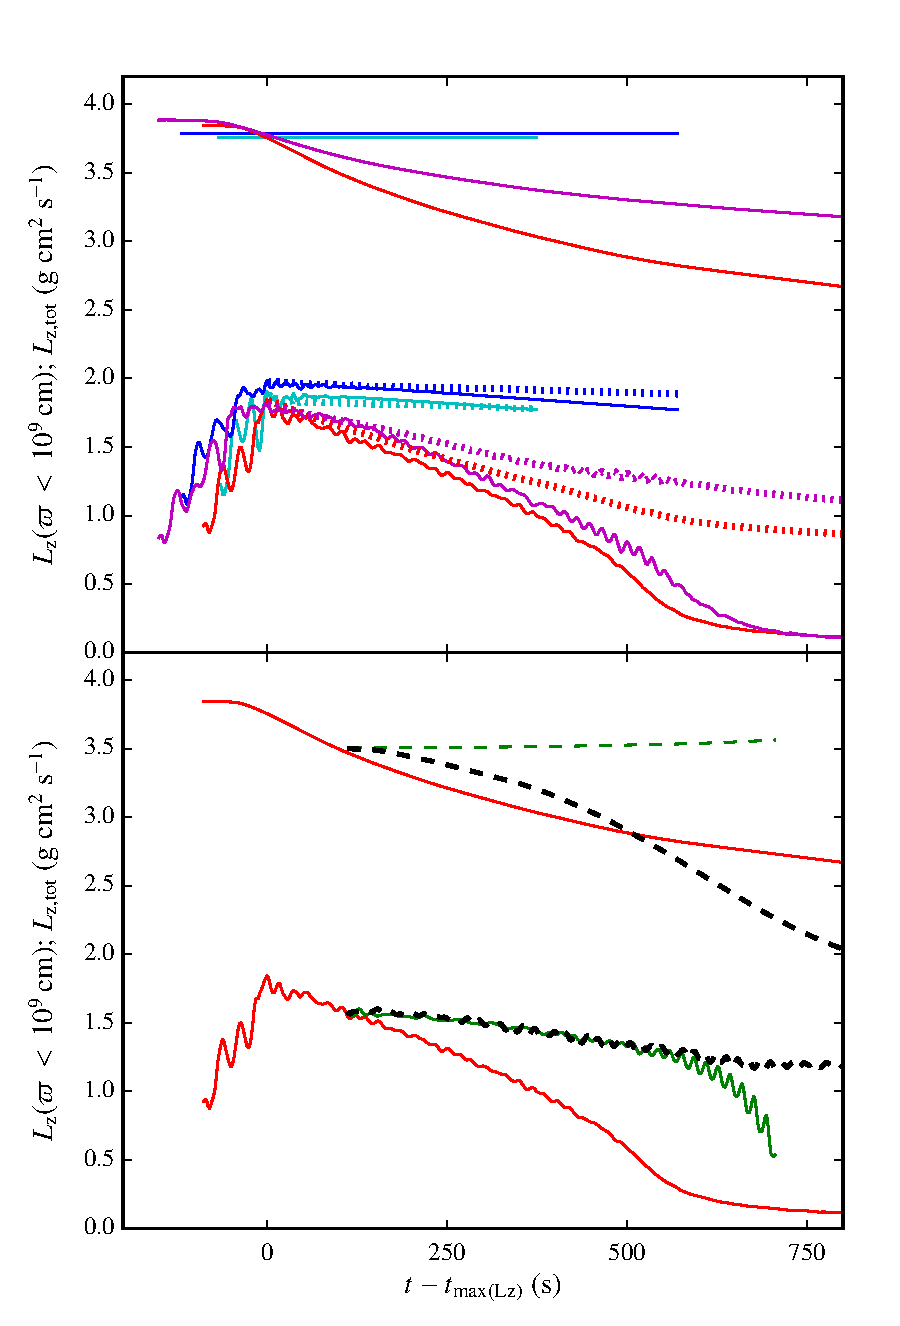
\includegraphics[angle=0,width=0.6\columnwidth]{chapter3_zhu+u/figures/lz_development.pdf}
\caption{Time evolution of total $z$-axis angular momentum \Lztot\ (top cluster of lines in each panel) and that within a cylinder of radius $\varpi = 10^9\,\mrm{cm}$, \Lzinner\ (bottom cluster), for various simulations in 2013-2014.  $t=0$ is defined as the time in each simulation when \Lzinner\ achieves its maximum value.  In the top panel, red and magenta lines represent the low and standard-resolution \arepo\ simulations, respectively, while the cyan and blue ones represents low and standard-resolution \gasoline\ ones, respectively.  Dotted lines represent angular momentum balance $\Lbal(\winnercyl)$, which should be flat in the absence of spurious angular momentum losses; colors correspond to their respective simulations.  Different initial amounts of total angular momentum between \arepo\ and \gasoline\ runs is due to inconsistencies in their initial conditions that have subsequently been solved.  In the bottom panel, the red line is again the low-resolution \arepo\ simulation, while the green line is for an \arepo\ low-resolution run where the mesh is held static after $t = 114\,\mrm{s}$ (dotted line represents angular momentum balance).  The dashed black line is a \flash\ simulation that uses the \arepo\ low-resolution run at $t = 114\,\mrm{s}$ for initial conditions; its loss of total angular momentum is due to having outflow boundaries.}
\label{fig:c3_fix_angmo}
\end{figure}

In the top panel of Fig. \ref{fig:c3_fix_angmo}, we plot both the total $z$-axis angular momentum \Lztot\ and that within a cylinder oriented along the rotational axis and with radius \innercyl, which we denote \Lzinner, for low-resolution ($1\times10^{28}\,\mrm{g}$, or $2.5\times10^{5}$ particles/cells at the start of simulation) and standard-resolution ($2\times10^{27}\,\mrm{g}$) \gasoline\ and \arepo\ simulations.  Because coalescence occurs at different times between them, we shift each simulation's curve so that $t = 0$ corresponds to the ``coalescence time'', defined as the time in each simulation when \Lzinner\ achieves its maximum value.  SPH formally conserves angular momentum, and we find the \Lztot\ for \gasoline\ varies in time by $\lesssim10^{-5}$ its mean value at either resolution.  On the other hand, the \arepo\ low-resolution simulation loses a \textit{third} of its angular momentum over $\sim1000\,\mrm{s}$, and the standard-resolution one $\sim20$\%.  

% Arepo doesn't have a fixed resolution, and so the number of mesh generating points will increase with time.  The low-res NoVolRef run on magny starts at 255,035 and and ends at 1000 s with 6,397,501 points (remember to remove the background grid with dc.d["backgrid"] < 0.5!).  The high-res one starts at 1,275,092 points and ends with 1,607,823 points.

A moving mesh that refines in regions of high density may not properly resolve the outer regions of the simulation, where the momentum appeared to be carried, nor low-density but high-energy (and thus dynamically important) regions near the center, such as the hot, low-density vortex encapsulated by the dense crescent.  To better poinpoint where in the system the angular momentum is being spuriously lost, we compute (similar to \cite{ji+13} Sec. 2.2.4) the theoretically expected change in $z$-angular momentum.  For a cylinder $V$ oriented along the rotational axis, this is given by (via the Euler equations)

\eqbegin
\frac{\ptl \Lz}{\ptl t} = - \oint_V \rho \varpi v_\phi v_\varpi dS + \int_V {\bf \varpi}\times{\bf \nabla}\Phi dV
\label{eq:c3_angmobalance}
\eqend

%\eqbegin
%\frac{\ptl L_i}{\ptl t} = - \oint_V \epsilon_{ijk} \rho x^ju^k u_l dl^l + \int_V \epsilon_{ijk} x^j F^k dV - \int_V \epsilon_{ijk} x^j \ptl^kP dV
%\label{eq:angmobalance}
%\eqend

% PROOF PRESSURE TORQUE IS ZERO (http://adama.astro.utoronto.ca/~cczhu/mergerwiki/doku.php?id=nov2013&#november_8th):
%\begin{eqnarray}
%\left(\int_V \epsilon_{ijk} x^j \partial^kP dV\right)_z &=&\int_r\int_\phi r \frac{\partial P}{\partial \phi} rdrd\phi \nonumber \\
%&=& \int_r r^2 (\int_\phi \frac{\partial P}{\partial \phi} d\phi)dr \nonumber \\
%&=& \int_r r^2 (P(2\pi) - P(0))dr \nonumber \\
%&=& 0 \nonumber
%\end{eqnarray}

\noindent where the first term encapsulates advection (including wave motion; eg. \citealt{balb03}) out of the volume and the second external torque -- in our case gravitational.\footnote{A third, pressure torque term also arises in general, but for an axisymmetric volume it is analytically zero (and numerically negligible as well).}  Subtracting the time-integral of Eqn. \ref{eq:c3_angmobalance} (i.e. the cumulative angular momentum change $\Delta \Lz$) from the volume's angular momentum gives us the ``balance''

\eqbegin
\Lbal(t) = L(t) - \Delta \Lz = L(t) - \int_{t_0}^{t}\frac{\ptl \Lz}{\ptl t'}dt'.
\eqend

\noindent In a system with perfect angular momentum conservation, $\Lbal(t) = \Lbal(t_0)$.  In Fig. Fig. \ref{fig:c3_fix_angmo} \Lbal\ for a cylinder of $\varpi = 10^9\,\mrm{cm}$ is plotted as a dashed line for each simulation.  While $\Lbal(\winnercyl)$ decreases by $\sim5$\% for the \gasoline\ simulations (likely due to artificial viscosity, not included in Eqn. \ref{eq:c3_angmobalance}), the change in \Lbal\ accounts for approximately \textit{all} of the total spurious losses in \arepo\ (compare the \Lztot\ and \Lbal\ lines), invalidating the hypothesis that it is the outer regions of the simulation spuriously losing angular momentum.  

% Arepo Lz losses determined by taking the first and last points in the balance.p files, eg. "arl_old.d["Lz"][-1,-1]/arl_old.d["Lz"][0,-1]"

To test whether the low-density, high-energy regions near the center were underresolved, we added a volume refinement criterion for cells within $\varpi\,=\,10^9\,\mrm{cm}$ that activates once more than $75$\% of the system's mass is within this boundary; This translated to a dramatic increase in resolution over time, with the simulation eventually exceeding $2\times10^7$ grid points.  This run loses $\sim5$\% of \Lztot\ in $\sim500\,\mrm{s}$, but $\sim30$\% of \Lzinner\ is still spuriously lost over the same timespan, meaning spurious losses would only be rendered negligible at impractically high resolutions.

% From Phil Chang: "The grid that I used was an outer grid of 256^3 in a box whose size was 1.6e5 km on the side (\Delta x = 624 km).  Two refined grids were deployed.  First level of refinement was at a scale < 50000 km from the center and a factor of 4 enhancement (Delta x = 156 km).  Second level was at a scale of 30000 km from the center and was a factor of 2 enhancement in resolution (Delta x = 78 km).  The second level basically covered the remnant. Effective resolution was 2048^3.  Gravity was solved using the multipole method with an lmax=50 (check was used with a multigrid method and a multipole with lmax=200 and no real differences were found). Solver was unsplit with a HLLC Riemann solver for HD and HLLD for MHD."

In the bottom panel of Fig. \ref{fig:c3_fix_angmo}, we plot a simulation performed in the Eulerian code \flash\ (\citealt{fryx+00}, {\charles DUBEY+09 from KASHYAP+15}), using the low-resolution \arepo\ run at $t = 110\,\mrm{s}$ (chosen to be $\sim2$ orbital periods after coalescence) for initial conditions.  We used a 3D Cartesian grid of size $1.6\times10^{10}\,\mrm{cm}$ to a side, with multiple levels of fixed-mesh refinement centered on the newly-formed merger remnant such that its core is resolved with cells $7.8\times10^6\,\mrm{cm}$ to a side (comparable to low-resolution \arepo's $\sim10^7\,\mrm{cm}$ in the core).  Gravity was solved using the multiple solver with $l_\mrm{max} = 50$, and fluxes propagated with the HLLC Riemann solver.  We also plot a low-resolution \arepo\ run where, at $t = 110\,\mrm{s}$ the mesh's velocities were forced to zero, transforming \arepo\ into a static grid code operating on an unstructured mesh.  Considering the sheer number of differences between the two codes, their simulations agree remarkably with one another on the rate of change of \Lzinner\ until very late times (when the remnant drifted away from the \arepo\ static mesh).  {\charles Both also conserve total angular momentum to within $\sim2$\%}, and $\Lbal(\winnercyl)$ for the \arepo-static run changes by $\sim1$\% over $\sim500\,\mrm{s}$.\footnote{We also attempted to transport \arepo\ simulation snapshots following coalescence into \gasoline, and vice versa.  The former showed angular momentum transport and the spiral pattern fading away within $\sim150$ s, while the latter showed the onset of Kelvin-Helmholtz instabilities at the interface between the rigidly rotating and sub-Keplerian portions of the remnant, followed by angular momentum loss.  This was the case even when the \gasoline\ initial conditions were nearly axisymmetric, and stable to hydrodynamic instability by \cite{maed+13}'s modified Solberg-H{\o}iland criterion.}  These simulations suggested \arepo's moving mesh scheme cause spurious angular momentum losses.

Eventually, two aspects of \arepo's original hydrodynamic scheme (Sec. \ref{ssec:c3_arepo}) responsible for making the code only \textit{first-order} convergent for non-trivial moving meshes were pinpointed and revised; this is detailed in \cite{pakm+15}, which we now summarize.  First, while Eqn. \ref{eq:c3_muscl_hancock} provides second-order covergence on static meshes of arbitrary geometry, it only uses the initial state of the mesh itself, and so only provides first-order convergence on moving meshes.  Second, \arepo's estimate for $\phi({\bf f}_{ij})$ in Eqn. \ref{eq:c3_gauss_green} assumes that the cell centers of mass ${\bf s}$, where the value of ${\bf W}$ is defined, and mesh-generating points ${\bf r}$ align, which is untrue for severely distorted meshes.  This first-order convergence does not inevitably cause major errors -- indeed, \cite{pakm+15} finds it does not affect their galaxy formation studies (eg. \citealt{XXX}) -- but for a rotation-dominated system being simulated over hundreds of dynamical times, such as the accretion disk in \cite{pakm+15}, systematic deviations in angular momentum conservation become apparent.

The solution is also two-fold: first, replace Eqns. \ref{eq:c3_arepo_timeadv} and \ref{eq:c3_muscl_hancock} by a hybrid MUSCL-RK2 method:

\begin{eqnarray}
{\bf W}^\prime_i &=& {\bf W}^n_i + \Delta t \, \frac{\ptl {\bf W}}{\ptl t} \nonumber \\
{\bf r}^\prime &=& {\bf r}^n +  \Delta t \, {\bf w}^n \nonumber \\
{\bf Q}^{n+1}_i &=& {\bf Q}^n_i - \frac{\Delta t}{2} \, \left( \sum_j A^n_{ij} {\bf \hat{F}}_{ij}^{n} \left( {\bf W}^n \right) + \sum_j A^\prime_{ij} {\bf \hat{F}}_{ij}^{\prime} \left( {\bf W}^\prime \right) \right) \nonumber \\
{\bf r}^{n+1} &=& {\bf r}^\prime,
\end{eqnarray}

\noindent where ${\bf r}$ is the coordinate of the mesh-generating point.  With this method, we first make a prediction of the cell's future primitive variables ${\bf W}^\prime$, as well as the future Voronoi mesh.  We then use both the current and predicted values to calculate an average flux and time-evolve the cell.  {\charles Spatial extrapolation to the cell interface is implicit when calculating $\hat{F}_{ij}$?}  The mesh velocities are assumed constant over $\Delta t$, so the predicted and true future mesh are identical.  Second, the Green-Gauss gradient estimate is replaced with linear least-squares estimator, where slope $\left\langle \nabla \phi \right\rangle_i$ is determined by minimizing

\eqbegin
\sum_j g_j \left(\phi_j - \phi_i - \left\langle \nabla \phi \right\rangle_i({\bf s}_j - {\bf s}_i)\right)^2,
\label{eq:c3_leastsq_grad}
\eqend

\noindent where $g_j \equiv A_{ij}/|{\bf s}_j - {\bf s}_i|^2$ is a weighting function.  This estimate gives the value that best reproduces the change in $\phi$ when travelling from cell $i$ to any of its neighbours, and relies only on cell centers of mass (and their values of ${\bf W}$), rather than mesh generating points.  Working in concert, these ``RKLSF'' fixes allow \arepo\ to become second-order convergent.

\begin{figure}
\centering
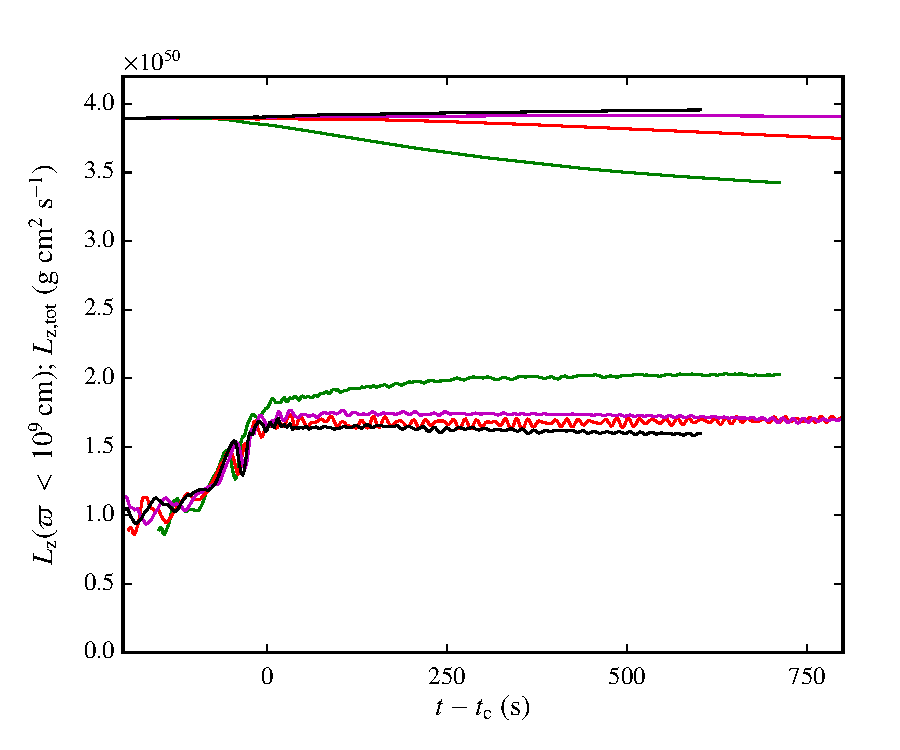
\includegraphics[angle=0,width=0.6\columnwidth]{chapter3_zhu+u/figures/lz_development2.pdf}
\caption{Time evolution of total $z$-axis angular momentum \Lztot\ (top cluster of lines) and that within a cylinder of radius $\varpi = 10^9\,\mrm{cm}$, \Lzinner\ (bottom cluster) for the \arepo-RKLSF simulations.  Colors indicate initial resolution: green is for $5.1\times10^4$ cells, red for $2.5\times10^{5}$, magenta for $1.3\times10^{6}$ and black for $2.5\times10^6$.}
\label{fig:c3_fix_angmo_nar}
\end{figure}

In Fig. \ref{fig:c3_fix_angmo_nar}, we show angular momentum evolution for \arepo-RKLSF runs (from Sec. \ref{ssec:c3_restest}) at resolutions ranging from $5.1\times10^4$ to $2.5\times10^6$ cells.  In all but the the lowest-resolution run, \Lztot\ deviates by less than $\sim7$\% from its initial value, and at the highest resolution run of $2.5\times10^6$ cells, it deviates by $\sim1$\% over $\sim840\,\mrm{s}$, an order of magnitude better than the $2\times10^7$-cell simulation without the RKLSF implementation.  Also, in all but the the lowest-resolution run, the spin-down of the remnant core is orders of magnitude slower (discussed further in Sec. \ref{ssec:c3_results}), cementing the fact that the rapid spin-down seen in Fig. \ref{fig:c3_fix_angmo} was an artefact of spurious angular momentum losses.  We now compare these \arepo-RKLSF simulations against ones in \gasoline.

%\noindent where $e = e_\mathrm{int} + \frac{1}{2}v^2$.  This states that the conserved quantities ${\bf U}$ are modified with the divergence of the flux function ${\bf F(U)}$; we can then discretize the whole thing as $\Delta{\bf U} = -\Delta t {\bf A}\cdot{\bf F(U)}$, where ${\bf A}$ is the size of a cell wall (pointed in the surface normal direction).  We then define ${\bf Q}_i = \int_V{\bf U}dV$ to be the value of ${\bf U}$ within a cell; this is effectively the value of ${\bf U}$ at the CM.  We get

%\eqbegin
%{\bf Q}_i^{n+1} = {\bf Q}_i^n - \Delta t \sum_jA_{ij}{\bf \hat{F}}_{ij}^{n+1/2}
%\eqend

%\noindent Arepo doesn't use ${\bf U}$, but rather

%\eqbegin
%{\bf W} = 
%\left( \begin{array}{c}
%\rho \\
%{\bf v} \\
%P \end{array} \right)
%\eqend

%\noindent the conversion to which you can find in the MergerWiki.  The tradition MUSCL-Hancock scheme uses a slope-limited piecewise linear spatial reconstruction as well as a first-order time-extrapolation by half a timestep:  

%\eqbegin
%{\bf W}_\mathrm{cell-wall} = {\bf W}_\mathrm{center} + {\bf \frac{\partial W}{\partial r}}({\bf r}_\mathrm{cell-wall} - {\bf r}_\mathrm{center}) + {\bf \frac{\partial W}{\partial t}}\frac{\Delta t}{2}
%\eqend

%\noindent A Riemann solver is then used to calculate the fluxes between cells and find ${\bf F}({\bf U})$.  For standard Arepo, spatial gradients of any conserved quantity $\phi$ are calculated using the Green-Gauss estimate,

%\eqbegin
%   \left< \nabla \phi \right>_i = \frac{1}{V_i} \sum_j A_{ij} \left( \left[ \phi_j - \phi_i \right] \frac{ \textbf{c}_{ij} }{ r_{ij} }
%   - \frac{ \phi_i + \phi_j }{2} \frac{ \textbf{r}_{ij} }{ r_{ij} } \right),
%\eqend

%\noindent where 

%\eqbegin
%   \textbf{c}_{ij} = \frac{1}{A_{ij}} \int_{A_{ij}} \left( \textbf{r} - \frac{\textbf{r}_i + \textbf{r}_j}{2} \right) \mathrm{d}A
%\eqend

%\noindent this estimate works fine if the values ${\bf Q}$ are sampled at the mesh-generating points.  In practice the CM is only $\sim1$\% away from the mesh generating point.

%\item Recent experience with running stellar binary mergers, and experiments with the Yee vortex, have shown the Arepo is only first-order accurate in many general problems.
%\item There are two root causes.  The first is that, during time integration, the fluid variables themselves are advanced a half timestep (by estimation, of course).  However, the mesh is not, meaning the shape and orientation of $A_{ij}$ is correct only to first order.  The second is the deviation of the mesh-generating point away from the centre of mass in distorted meshes.
%\item The first issue can be fixed without a significant penalty in increased computation costs by replacing the MUSCL-Hancock scheme with a 2nd order Heun's method (a type of RK2 method), i.e. $y^{n+1} = y^{n} + \frac{\Delta x}{2}(f(y^n, x) + f(y', x'))$, and $y' = y^n + \Delta x f(y^n,x)$ and $x' = x + \Delta x$ are 1st order estimates of the next step.  That is,

%\begin{eqnarray}
%   \textbf{Q}^\prime_i &=& \textbf{Q}^n_i - \Delta t \sum_j A^n_{ij} \mathbf{\hat{F}}_{ij}^{n} \left( \textbf{U}^n \right)
%   \label{eqn:heunorig} \\
%   \textbf{r}^\prime &=& \textbf{r}^n +  \Delta t \, \textbf{w}^n \\
%   \textbf{Q}^{n+1}_i &=& \textbf{Q}^n_i - \nonumber \\
%   &&\frac{\Delta t}{2} \, \left( \sum_j A^n_{ij} \mathbf{\hat{F}}_{ij}^{n} \left( \textbf{U}^n \right) + 
%   \sum_j A^\prime_{ij} \mathbf{\hat{F}}_{ij}^{\prime} \left( \textbf{U}^\prime \right) \right) \label{eqn:heunupdate} \\
%   \textbf{r}^{n+1} &=& \textbf{r}^n + \frac{\Delta t}{2} \, \left( \textbf{w}^n + \textbf{w}^n \right) = \textbf{r}^n +  \Delta t \, \textbf{w}^n.
%\end{eqnarray}

%\noindent The trick here is that ${\bf r}' = {\bf r}^{n+1}$, so the mesh for the ${\bf F}_{ij}'$ estimate is simply the mesh at the next timestep.  In practice calculating the intermediate state ${\bf Q'}$ is problematic, so we estimate it in the same way we estimate the half-timestep extrapolation in the MUSCL-Hancock scheme:

%\begin{eqnarray}
%   \textbf{W}^\prime_i &=& \textbf{W}^n_i + \Delta t \, \frac{\partial \textbf{W}}{\partial \textbf{t}}
%   \label{eqn:heunnew} \\
%   \textbf{r}^\prime &=& \textbf{r}^n +  \Delta t \, \textbf{w}^n \\
%   \textbf{Q}^{n+1}_i &=& \textbf{Q}^n_i - \nonumber \\
%   &&\frac{\Delta t}{2} \, \left( \sum_j A^n_{ij} \mathbf{\hat{F}}_{ij}^{n} \left( \textbf{W}^n \right) + 
%   \sum_j A^\prime_{ij} \mathbf{\hat{F}}_{ij}^{\prime} \left( \textbf{W}^\prime \right) \right) \\
%   \textbf{r}^{n+1} &=& \textbf{r}^n +  \Delta t \, \textbf{w}^n.
%\end{eqnarray}

%\item The second issue can be fixed by using a (second-order) local least squares fit.  The method assumes that a conserved quantity $\phi$ can be approximated anywhere within the cell by

%\eqbegin
%   \phi \left( \textbf{r} \right) = \phi \left( \textbf{s}_i \right) + \left< \nabla \phi \right>_i \cdot \left( \textbf{r} - \textbf{s}_i \right)
%\eqend

%\noindent where ${\bf s}_i$ is the value of $\phi$ at the cell $i$ CM.  Since we know the values of $\phi$ at all neighbouring cell CMs, we can write:

%\eqbegin
%   \phi_j = \phi_i + \left< \nabla \phi \right>_i \left( \textbf{s}_j - \textbf{s}_i \right).
%\eqend

%\noindent For a cell with multiple neighbours, $\left< \nabla \phi \right>_i$, which only has three components in 3D, will be highly overdetermined.  We therefore can determine a best fit for $\left< \nabla \phi \right>_i$ by minimizing the deviation parameter:

%\eqbegin
%   \mathrm{S_{tot}} = \sum_j g_j \left( \phi_j - \phi_i  - \left< \nabla \phi \right>_i \left( \textbf{s}_j - \textbf{s}_i  \right) \right)^2.
%\eqend

%\item Convergence tests show that these two fixes combined allow Arepo to achieve second-order convergence.  Real-world testing show substantial improvement for angular momentum conservation in stellar binary mergers, but little effect on galaxy formation simulations.

